{ %section8_1
	\subsection{Порядок выполнения работы}
	\Large
	\begin{enumerate}
		\itemНа языке Си написать программу для вычисления числа A по формуле:
			$$A\;=\;2\;\cdot\;\frac2{\sqrt2}\;\cdot\;\frac2{\sqrt{2\;+\;\sqrt2}}\;\cdot\;\frac2{\sqrt{2\;+\;\sqrt{2\;+\;\sqrt2}}}\;\cdot\;\dots,$$
			 при этом пусть в вычислении используется N первых множителей, где N должно задаваться в программе в виде параметра.
		\itemПосле вычисления А программа должна вычислить число В по формуле: 
			$$B\;=\;\frac6A\;{\textstyle\prod_ {i=1}^M}\left(\frac{2i\;+\;3}{2i\;+\:1}\right)^{2i\;+\;1}\left(\frac i{i\;+\:1}\right)^{2i}$$
			при этом пусть в вычислении используется M первых множителей.
			\parДополнительные указания: в расчётах числа B не следует использовать целочисленное деление; программа должна использовать циклы for, записанные только в канонической форме; результаты вычисления А и В должны быть выведены в консоль:
			\begin{figure}[H]
				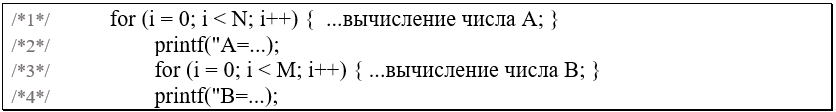
\includegraphics[width=1\linewidth]{lab5Example1}
			\end{figure}
			\parДополнительные указания: в расчётах числа B не следует использовать целочисленное деление; программа должна использовать циклы for, записанные только в канонической форме; результаты вычисления А и В должны быть выведены в консоль:
		\itemРаспараллелить программу из п.1, используя следующие директивы OpenMP:
			\begin{figure}[H]
				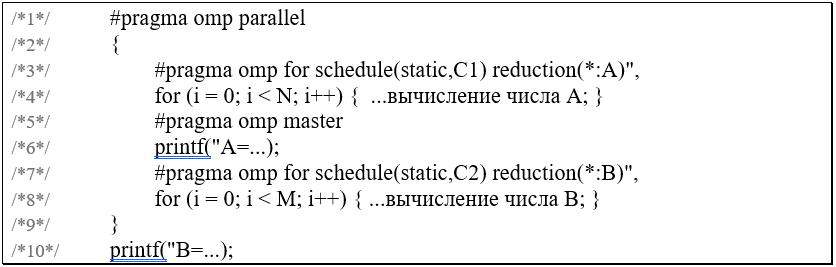
\includegraphics[width=1\linewidth]{lab5Example2}
			\end{figure}
			где значение C1 и C2 следует выбрать самостоятельно, приведя в отчёте обоснование сделанного выбора. Привести графики параллельного ускорения для различных N и M.
		\itemПереписать программу из п.2, используя Pthreads вместо OpenMP. Способ распараллеливания должен быть идентичен тому, что используется  в п.2. Дополнительные указания: для реализации операции, соответствующей OpenMP-директиве reduction(...), следует использовать Pthreads-мьютекс; перед выводом числа А на экран следует использовать функцию pthread\textunderscore barrier\textunderscore wait; перед выводом числа В на экран следует использовать pthread\textunderscore join.
		\itemПровести сравнительный анализ программы из п.2 и п.3 (сравнить размер исполняемого файла, параллельное ускорение для разных N и M, количество строк кода, добавленного при распараллеливании и прочее).
		\itemЗадание на "четвёрку" и "пятёрку": параллельное ускорение в п.2 и п.4  должно быть измерено в виде доверительного интервала с доверительной вероятностью 0.95.
		\itemЗадание на "пятёрку": вместо директивы schedule(static...) в п.2 и п.3 следует использовать директиву schedule(dynamic...), если итерации внутри соответствующего цикла различаются по сложности вычислений.
	\end{enumerate}
}